\section{Requisiti e casi d'uso}

\subsection{Use cases}
Di seguito sono riportati i requisiti del sistema che si vuole implementare. Per ciascun caso si indica
il codice del caso d'uso, il titolo e la user story al fine di facilitare la comprensione.

\begin{itemize}
    \item \textbf{UC1 - Login}. Come utente voglio accedere al mio account;
    \item \textbf{UC2 - Signup}. Come utente voglio potermi registrare al sistema;
    \item \textbf{UC3 - Logout}. Come utente voglio potermi disconnettere dal sistema;
    \item \textbf{UC4 - Visualizzazione iscrizioni}. Come utente voglio visualizzare gli eventi ai quali sono iscritto;
    \item \textbf{UC5 - Visualizzazione meteo}. Come utente voglio visualizzare il meteo entro 5 giorni dall’evento;
    \item \textbf{UC6 - Visualizzazione consigliati}. Come utente voglio poter visualizzare gli eventi consigliati;
    \item \textbf{UC7 - Ricerca eventi}. Come utente voglio poter cercare dei nuovi eventi, scegliendo degli opportuni parametri di ricerca;
    \item \textbf{UC8 - Visualizzazione risultati ricerca.} - Come utente, voglio poter visualizzare tutti i risultati della ricerca;
    \item \textbf{UC9 - Visualizzazione specifico risultato.} - Come utente, voglio poter consultare il singolo risultato della ricerca eseguita, visualizzando nei dettagli informazioni quali la località, la data e l’organizzatore;
    \item \textbf{UC10 - Iscrizione ad un nuovo evento.} Come utente, voglio potermi iscrivere ad uno degli eventi disponibili;
    \item \textbf{UC11 - Cancellazione iscrizione.} Come utente, voglio poter cancellare la mia iscrizione ad un evento;
    \item \textbf{UC12 - Visualizzazione partecipanti.} Come utente, voglio poter visualizzare gli utenti che parteciperanno ad un evento;
    \item \textbf{UC13 - Visualizzazione profilo utente.} Come utente, voglio poter visualizzare sul mio profilo le esperienze a cui ho preso parte e quelle a cui sono iscritto;
    \item \textbf{UC14 - Visualizzazione profilo organizzatore.} Come utente organizzatore, voglio poter visualizzare sul mio profilo gli eventi passati da me organizzati e quelli futuri;
    \item \textbf{UC15 - Algoritmo iscrizione.} Come utente, voglio che solo i profili più adeguati possano partecipare ad un evento, e che solamente gli N profili più adeguati vengano accettati;
    \item \textbf{UC16 - Dettagli evento.} Come utente, voglio poter visualizzare tutte le informazioni relative all’evento per poter valutare se iscrivermi o meno;
    \item \textbf{UC17 - Eliminazione evento.} Come organizzatore voglio poter cancellare un evento che ho creato;
    \item \textbf{UC18 - Creazione evento.} Come organizzatore voglio poter creare un evento;
    \item \textbf{UC19 - Visualizzare profilo partecipanti.} Come utente voglio poter visualizzare il profilo di coloro che sono iscritti a un evento;
    \item \textbf{UC20 - Cambiare la foto del profilo.} Come utente voglio poter cambiare la mia foto di profilo;
    \item \textbf{UC21 - Cambiare la foto di copertina.} Come utente voglio poter cambiare la foto di copertina del mio profilo.
    \item \textbf{UC22 - Cambiare la foto di un evento.} Come organizzatore voglio poter cambiare la foto che descrive un mio evento.
\end{itemize}
\clearpage

\subsection{Priorità dei casi d'uso}

I casi d'uso possono essere ripartiti all'interno di tre code, a seconda della loro priorità nel processo di sviluppo.
\begin{itemize}
    \item Coda ad alta priorità: contiene i requisiti ritenuti fondamentali per il funzionamento dell'applicativo, ossia la creazione dei profili utente, la creazione di nuovi eventi ed il sistema di iscrizione agli eventi stessi. Saranno i primi use case implementati sia lato client che server;
    \item Coda a media priorità: coda contenente funzionalità di supporto, principalmente legate alla visualizzazione di informazioni ulteriori riguardo agli utenti e/o agli eventi;
    \item Coda a bassa priorità: coda nella quale vengono indicate le funzionalità meno rilevanti, non è prevista la loro implementazione tuttavia potremmo decidere di implementarli in base a come procederà il progetto.
\end{itemize}

In particolare, nelle tabelle di seguito [\ref*{tab: alta-priorità},\ref*{tab: media-priorità},\ref*{tab: bassa-priorità}] 
è possibile osservare come i casi d'uso precedentemente individuati possano essere suddivisi.
\clearpage

\begin{table}
\begin{center}
\begin{tabular}{ |c|c|}
 \hline
 \textbf{NUMERO}& \textbf{TITOLO} \\ \hline
 UC1& Login\\ \hline
 UC2& Signup\\ \hline
 UC3& Logout\\ \hline
 UC7 & Ricerca eventi \\ \hline
 UC8 & Visualizzazione risultati ricerca \\ \hline
 UC9 & Visualizzazione specifico risultato \\ \hline
 UC10 & Iscrizione ad un nuovo evento\\ \hline
 UC11 & Cancellazione iscrizione\\ \hline
 UC15& Algoritmo iscrizione\\ \hline
 UC17& Eliminazione evento\\ \hline
 UC18& Creazione evento\\ \hline
\end{tabular}
  \caption{Coda ad alta priorità}
  \label{tab: alta-priorità}
\end{center}
\end{table}

\begin{table}
\begin{center}
\begin{tabular}{ |c|c|}
 \hline
 \textbf{NUMERO}& \textbf{TITOLO} \\ \hline
 UC5& Visualizzazione meteo\\ \hline
 UC6& Visualizzazione consigliati\\ \hline
 UC13&Visualizzazione profilo utente\\ \hline
 UC14&Visualizzazione profilo organizzatore\\ \hline
 UC16& Dettagli evento\\ \hline
\end{tabular}
  \caption{Coda a media priorità}
  \label{tab: media-priorità}
\end{center}
\end{table}

\begin{table}
\begin{center}
\begin{tabular}{ |c|c|}
 \hline
 \textbf{NUMERO}& \textbf{TITOLO} \\ \hline
 UC4& Visualizzazione iscrizioni\\ \hline
 UC12& Visualizzazione partecipanti\\ \hline
 UC19& Visualizzare profilo partecipanti\\ \hline
 UC20& Cambiare la foto del profilo\\ \hline
 UC21& Cambiare la foto di copertina\\ \hline
 UC22& Cambiare la foto di un evento\\ \hline
\end{tabular}
  \caption{Coda a bassa priorità}
  \label{tab: bassa-priorità}
\end{center}
\end{table}

\clearpage
\subsection{Use case diagram}
I requisiti precedentemente elencati possono essere visualizzati graficamente tramite l'use case diagram riportato in figura.

\begin{figure}[ht!]
    \centering
    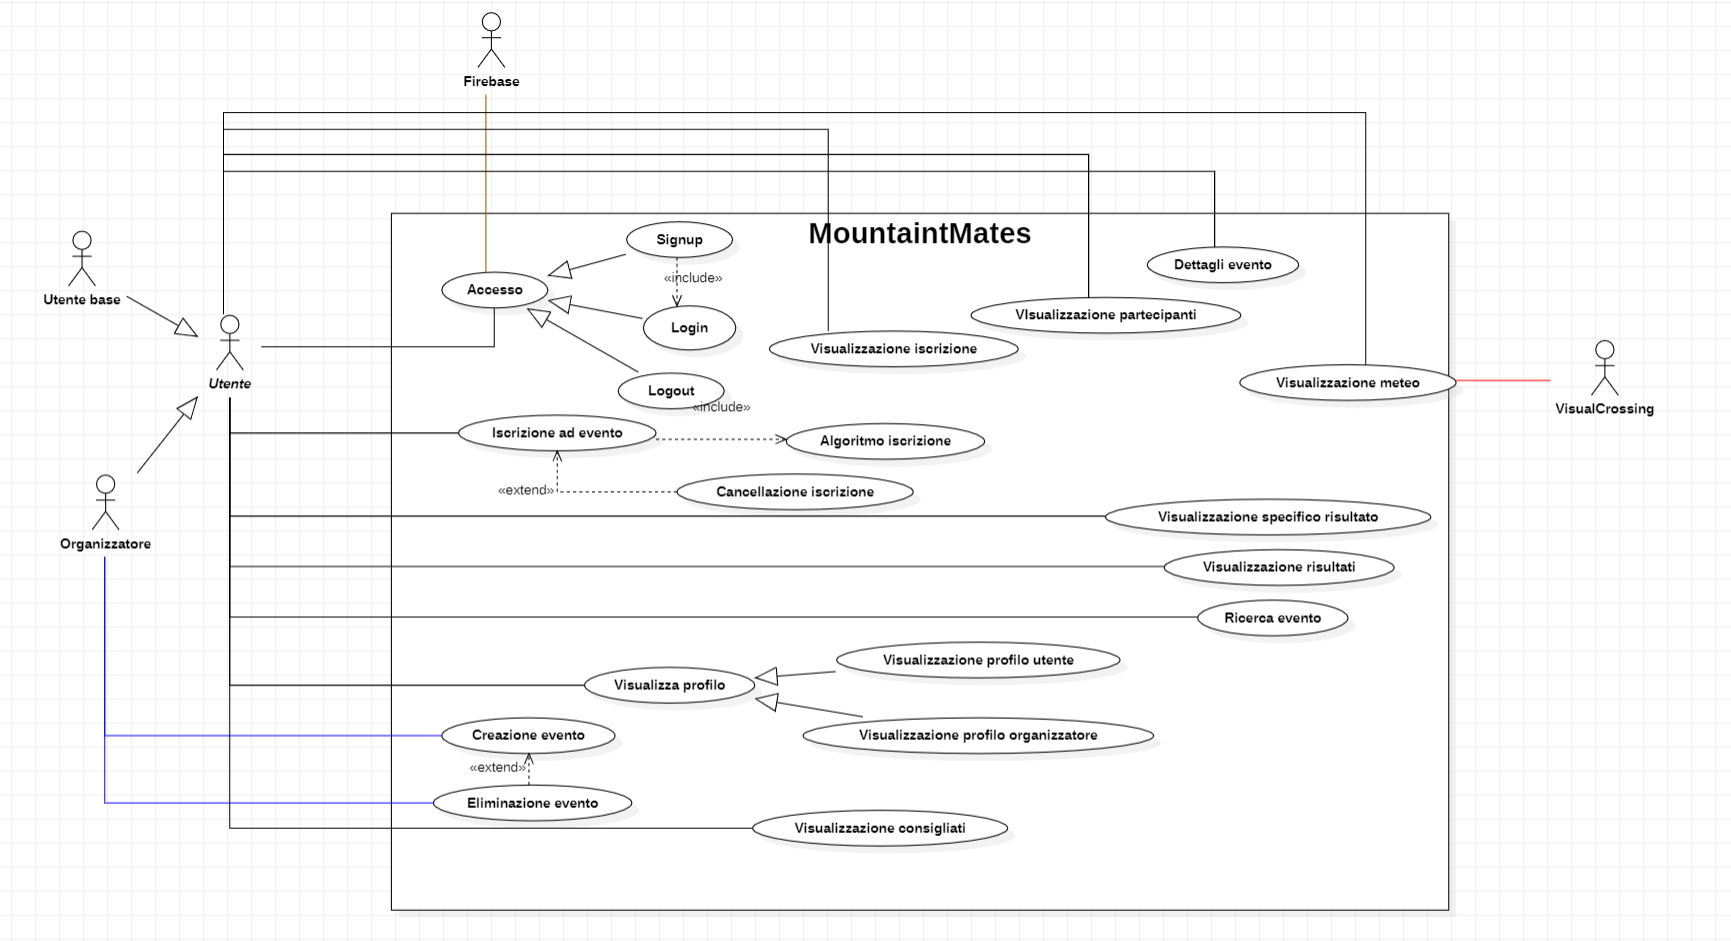
\includegraphics[scale=0.55]{immagini/UseCases.png}
    \caption{Use cases}
    \label{fig: usecases}
  \end{figure}

E' stata introdotta una generalizzazione sugli utenti per distinguere le funzionalità accessibili da un utente base
rispetto a quelle di un organizzatore.
I due attori Firebase e VisualCrossing sono coinvolti nei casi d'uso relativi all'autenticazione ed alla visualizzazione delle
condizioni meteo sul luogo dell'evento.

Inoltre, l'iscrizione ad un evento richiede l'esecuzione del caso d'uso algoritmo di iscrizione in quanto, come detto precedentemente,
una volta raggiunto un massimo di iscritti solamente i primi N più qualificati saranno accettati all'evento.